\section{Ergebnis}
Schluss endlich haben wir eine uns mit Python eine Datenbank aufgebaut. Dies haben wir mit erst mit der Planung und dann mit der Ausführung bewältigt. Zu nächst haben wir uns die Daten angeguckt. Dann haben wir daraus ein ER-Modell erstellt und dies in ein relationales Schema gebracht. Dieses Schema haben wir dann verschmolzen um die letzte theoretische Übersicht der Datenbank aufzuzeigen. Darauf hin haben wir uns Anomalien angeguckt und Normalformen um diese zu verhindern. Danach haben wir uns die eigentliche Erstellung der Datenbank angeguckt und wie man mit SQL eine Tabelle einfügt. Nun haben wir die Daten nur noch eingefügt und abgespeichert. 

Dieses Einfügen klappt mit einer Geschwindigkeit von 40-60 Transaktionen die Sekunde, dass heißt nur für grob 5 Millionen Publikationen würden wir 100.000 Sekunden brauchen das sind 1667 Minuten oder auch ca. 28 Stunden. Davon abgesehen das noch 2 Millionen Autoren da zu kommen. Dazu kommt noch das Transaktionen nicht nicht Publikationen pro Sekunde sind, denn in Publikationen sind alleine zwischen 2-4 Autoren beteiligt die jedes mal Abgefragt werden müssen ob sie Existieren und wenn nicht angelegt werden. Hier müssen natürlich auch die Relationen angelegt werden die die beiden Tabellen verbindet. Daraus werden dann pro Publikation dann mindestens 6 Transaktionen mehr. Dazu kommen noch die ein bis zwei elektronischen Versionen pro Publikation mit den Relationen. Somit landen wir grob bei einer Dauer von 308 Stunden das sind fasst 13 Tage. Da durch viele erneute Anpassungen der Datenbank dieser Prozess wiederholt werden musste, werden hier nur Ausschnitte der bisherigen Ergebnisse gezeigt. 

Dazu verwenden wir Data Querie Language(DQL) eine Datenabfragesprache die wieder ein Teil von SQL da stellt. Hiermit können wir Anfragen an die Datenbank stellen die uns dann dem entsprechende Antworten liefert. Mit diesem Teil von SQL kann in der Datenbank nichts geändert werden weder Struktur noch Daten.

\begin{figure}[!htb]
	\centering
	%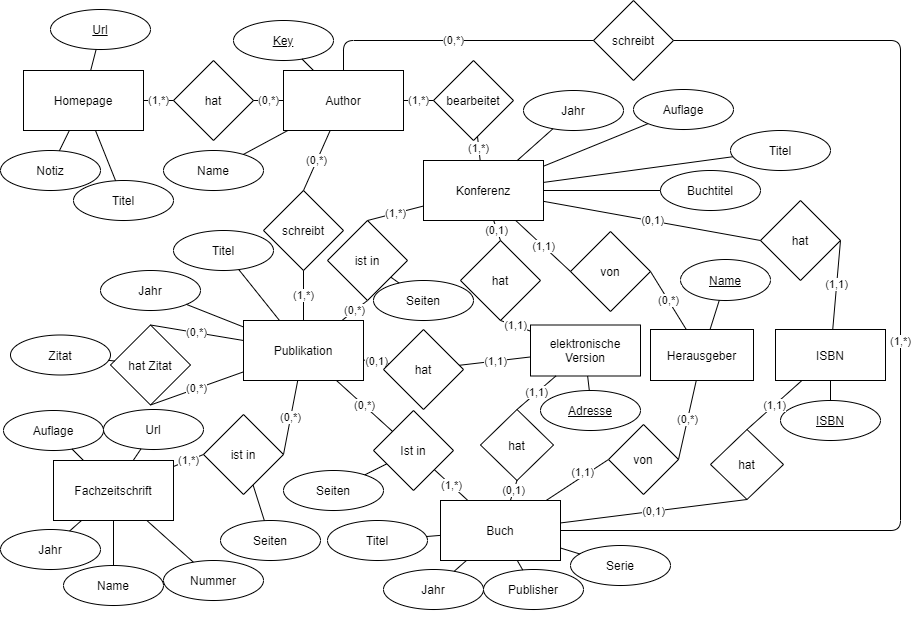
\includegraphics[width=14cm,keepaspectratio]{ER-Modell}
	\caption{DQL Beispiel}
	\label{fig:dqlbeispiel}
\end{figure}

Erklärung...%todo

\begin{figure}[!htb]
	\centering
	%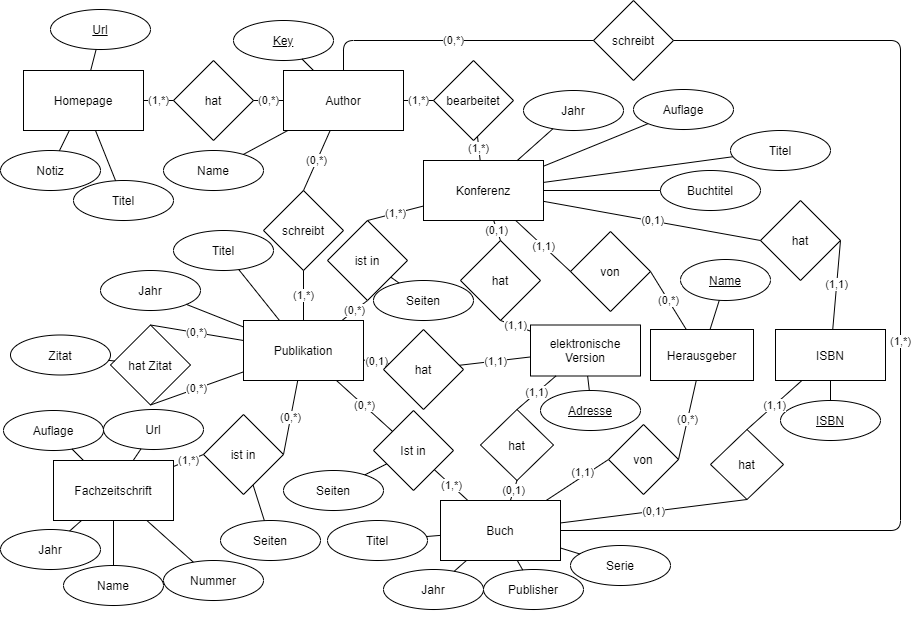
\includegraphics[width=14cm,keepaspectratio]{ER-Modell}
	\caption{DQL Ergebnis}
	\label{fig:dqlergebnis}
\end{figure}